% Chapter Template

\chapter{Construcción y evaluación de la gramática}

\label{Chapter4} % Change X to a consecutive number; for referencing this chapter elsewhere, use \ref{ChapterX}

%----------------------------------------------------------------------------------------
%  SECTION 1
%----------------------------------------------------------------------------------------

\section{Reglas de la gramática}

Como se mencionó en la sección anterior, se puede utilizar un generador de lenguaje natural o verbalizador basado en plantillas (template-based \textbf{natural language generation}). Es necesario en este punto construir templates que representen la manera más usual \textbf{o natural} de leer expresiones matemáticas \textbf{de manera que se construyan frases fidedignas al original y fáciles de comprender cuando se lean en voz alta por un lector de pantalla}. Para ello se contactó a distintos estudiantes de carreras matemáticas, e incluso Ingenieros en Sistemas y Lic. en Cs de computación para poder reconocer las distintas maneras de leer una expresión. Todas las representaciones fueron tomadas en cuenta, dado que todas ellas describen las expresiones matemáticas dependiendo de quién la puede leer.\\

Las fórmulas matemáticas pueden leerse dependiendo del contexto geográfico, de la edad, de la convención utilizada en la institución educativa, de distintos libros se puede llegar a la conclusión que no hay una única manera de representar mediante texto una misma fórmula matemática.
Por ejemplo,

$$\frac{a}{b}$$

Puede leerse de distintas formas, por ejemplo, \textit{a sobre b}, \textit{a dividido b}, \textit{la fracción de a y b}, \textit{a partido por b}. Por lo tanto, es necesario conocer las distintas alternativas de la gramática.\\

Dado que se utiliza un template como gramática de generador de lenguaje, es fácil de añadir y extender a nuevas producciones si alguna no se encontrase disponible o las disponibles son incorrectas.\\

\section{¿El resultado es la representación más usual?: Evaluación}

La evaluación de estos sistemas es un campo muy vital tanto para determinar cuán efectivo es nuestro sistema y además de optimizarlo en caso de alguna oportunidad de mejora. La naturaleza del prototipo desarrollado en este trabajo permite hacer una anlogía con la traducción automática, donde el texto origen es la fórmula matemática en MathML y el texto meta o destino es la frase en lenguaje natural; de este modo se piensa TexToES como un traductor de matemática a español, y puede evaluarse utilizando conceptos tomados del área de la traducción automática, como se explica a continuación.

Muchas de las propiedades que conforman a la calidad de una traducción son:
\begin{itemize}
\item \textbf{Fidelidad}, busca responder a la pregunta: ¿la transcripción tiene el mismo significado que el idioma fuente?
\item \textbf{Comprensibilidad}, una transcripción puede ser correcta pero sin embargo difícil de entender, a veces más dificil que el idioma fuente.
\item \textbf{Fluidez}, la traducción puede tener el significado correcto y hasta fácil de entender, sin embargo, podría suceder que ningun usuario la menciona alguna vez.
\end{itemize}

Para evaluar TexToES se han encarado tres tipos de evaluaciones, aunque las tres en conjunto buscan medir y evaluar el sistema para adaptarse a mejores resultados y optimizaciones.

Se han desarrollado y usado métodos de evaluación que son humanos, automáticos y semiautomáticos (humanos presentes o automatización asistida).

Antes de comenzar el desarrollo de cualquier tipo de evaluación y también debido a la inexistencia de reglas para leer expresiones matemáticas, se ha realizado una encuesta que su objetivo fue el de reconocer las representaciones más usuales para distintas fórmulas matemáticas. Las encuestas consisten en mostrar al encuestado 3 fórmulas matemáticas y el sujeto debía de responder a la siguiente consigna:\\

\begin{tcolorbox}
Si tuvieras que dictar las siguientes fórmulas a alguien para que las escriba, ¿Cómo las dictarías?
La consigna es que escribas una descripción en texto de cómo leerías las siguientes fórmulas.

Por ejemplo, si la fórmula planteada es "(a + 2)/3 = f", podrías escribir algo así como "((a más 2) dividido 3) es igual a f".

- Escribir los números y fórmulas tal cual se presentan, como en el ejemplo.
- Agrupar con paréntesis el orden en que lo dictarías.
- Escribir "(" en lugar de "abrir paréntesis"
- Si no sabes cómo escribir una fórmula, simplemente omitila.
\end{tcolorbox}

Las encuestas se dividían por niveles, donde cada nivel contenía distintos tipos de expresiones.
En el nivel número uno, podíamos encontrar operaciones básicas como la suma, división, multiplicación, exponentes, raíces.
En el nivel dos, podíamos encontrar ya expresiones trigonométricas, funciones, derivadas, integrales.
En el nivel tres, podíamos encontrar sumatorias, productorias, matrices, etc.\\

De esta forma podemos aplicar un patrón de limpieza, donde no diferenciemos números, ni funciones, ni variables para poder quedarnos con producciones generales, y conocer desde distintas entradas recibidas en las encuestas cuáles son las posibles verbalizaciones para las distintas expresiones matemáticas.\\

Las encuestas han sido publicadas en distintos grupos y listas de distribución de FaMAF, y también ha sido difundida entre amigos y compañeros, alumnos y demás.

\section{Descripción del procedimiento}

El procedimiento consistió de distintas etapas, todas necesarias para evaluar la transcripción obtenida.

\begin{itemize}
\item Recolección de datos: Construcción y difusión del medio utilizado para obtener datos.
\item Pre-procesamiento de datos: Llevar los datos a un nivel general, para no distinguir entre números o nombres de variables. Además de estandarizar las respuestas para su fácil procesamiento.
\item Armado de Corpus (Corpus building): Reunión de los datos obtenidos, añadiendo información relevante tal como etiquetado y cantidad de ocurrencias.
\item Constructor de evaluadores: Construcción de distintos evaluadores que indiquen una métrica de confianza de la transcripción final. Tenemos un evaluador automático, semiautomático y manual.
\item Recolección de resultados: Presentación de resultados obtenidos y acciones tomadas.
\end{itemize}

\subsection{Recolección de datos}

Se ha utilizado \textbf{Google Forms} para crear los formularios que recolectaron la información necesaria que evidencie la forma más usual o natural de leer las fórmulas matemáticas.

Estos formularios contienen un total de 45 preguntas\cite{10} que abarcan distintos niveles de la matemática desde los operadores básicos como la suma y resta, hasta diferenciales. Un total de tres niveles y cinco encuestas cada uno presentando tres fórmulas.

Se ha recibido un total de 1298 respuestas de los distintos niveles. La tercera parte de las respuestas caen dentro del primer nivel. Mientras que último nivel ha obtenido menos de 100 respuestas en todas sus encuestas.

Todas las respuestas obtenidas pueden ser consultadas en el repositorio de esta tesis organizados por su respectivo nivel en un archivo de formato csv (comma separated values).

Cada archivo csv cumple con la siguiente estructura:\\
Una respuesta de un usuario está separada por comas (\textbf{,}) y el delimitador son las comillas dobles (\textbf{"}). Esto significa que todo carácter de \textbf{coma} dentro de dos comillas dobles no denotará una respuesta distinta.

En la primer línea están presentes los títulos de las preguntas y un dato adicional agregado por Google Forms que es el timestamp.

Ejemplo:\\
\textit{"Timestamp","¿Cómo la escribirías? n1.e2.f1","¿Cómo la escribirías? n1.e2.f2","¿Cómo la escribirías? n1.e2.f3"}

En las demás líneas se encuentran las respuestas.

Ejemplo:\\
\textit{"2015/11/24 9:07:45 PM GMT-3","r1","r2","r3"}

De esta forma podemos encontrar en los archivos csv en su primer columna la fecha en la que el usuario ha respondido, en su segunda columna la respuesta asociada a la primer pregunta, y así sucesivamente.

Una respuesta vacía implica la presencia de dos comillas dobles juntas (\textbf{""}).

\subsection{Pre-pocesamiento de datos}
Con el pre-procesamiento se intenta corregir o eliminar datos erróneos del conjunto de datos obtenidos. También se buscó la presencia de datos incompletos, inexactos, etc. y luego sustituir, modificar o eliminar estos datos sucios. Después de este pre-procesamiento, los datos podrán ser compatibles con el resto del sistema que evaluará la transcripción.

El pre-procesamiento se llevó a cabo teniendo en cuenta las siguientes consideraciones:

\begin{itemize}
   \item Eliminar todo character acentuado. Por ejemplo, el wording asociado al operador suma que puede ser \textbf{más} o \textbf{mas} a fines prácticos es el mismo.
   \item Con la misma razón anterior, se reemplazaron los nombres de variables, constantes y números por la palabra \textbf{\$VAR\$}. Porque para la verbalización de la suma, por ejemplo, podemos tener las siguientes instancias: 6 mas 5, 4 mas 9 y 7 sumado a 6. Nos interesa contar ambas primeras como la misma verbalización y diferenciarla de la segunda por contener otro wording.
   \item Corregir paréntesis para los casos que éstos no esten balanceados, no esten presentes o esten mal ubicados.
   \item Identificación de múltiples respuestas en una misma respuesta de formulario. Para estos casos, solo se trata cada respuesta como una instancia distinta.
\end{itemize}

Este comportamiento está implementado dentro de la clase \textit{lenguage\_evaluator} en el método \textit{prepare\_corpus} dentro del código fuente de este proyecto.

El método prepare\_corpus se encarga de revisar los archivos .csv obtenidos desde Google Forms, ejecutar las consideraciones descritas anteriormente y crear un archivo llamado \textbf{parsed\_responses.txt} con los datos limpios.

Para ver gráficamente su funcionamiento observemos la siguiente figura:

\begin{figure}[H]
\centering
  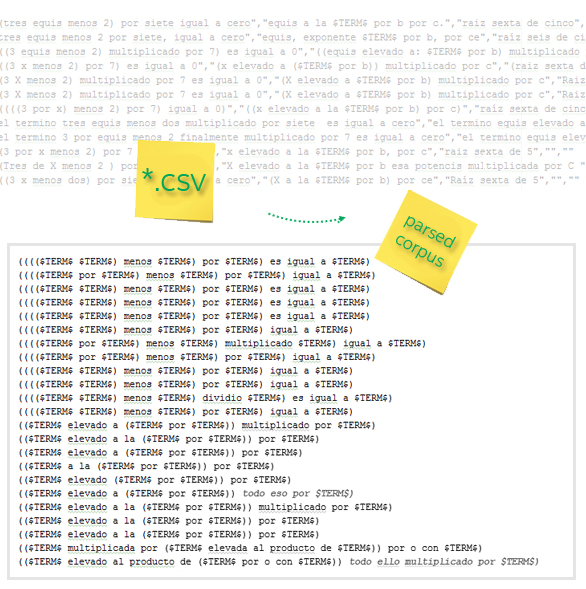
\includegraphics[width=11cm, height=11cm]{Figures/parsed_corpus}
  \caption[]{Funcionamiento de prepare\_corpus}
\label{fig:parsed_corpus}
\end{figure}

\subsection{Corpus building}

Esta parte del procedimiento se encarga de construir lo que será el corpus que se utilizará para hacer las evaluaciones de las transcripciones. En el corpus se reúne toda la información que los voluntarios dieron en su respuestas. Es información limpia y que puede exportarse para utilizarla en otro proyecto.

El comportamiento que describiré en esta sección puede encontrarse en el método \textbf{parse\_corpus} dentro de la misma clase.

Para crear el corpus simplemente se ha implementado un parser que sabe interpretar los datos limpios obtenidos por el punto anterior, para recolectar en un solo lado toda la información.

Este método se encarga de extraer de cada respuesta todas las estructuras gramaticales compuestas en él. Expliquemos esto mediante el siguiente ejemplo, supongamos:

\begin{tcolorbox}
input: ((\$TERM\$ elevado a (\$TERM\$ por \$TERM\$)) multiplicado por \$TERM\$)
output: []
\end{tcolorbox}

Nos posicionaremos entre el último paréntesis "(" y el primer paréntesis ")" a partir de él. Y extraemos eso como una regla gramatical atómica, reemplazandolo en la fórmula original como \$TERM\$.

\begin{tcolorbox}
input: ((\$TERM\$ elevado a \$TERM\$) multiplicado por \$TERM\$) \\
output: [(\$TERM\$ por \$TERM\$), ]
\end{tcolorbox}

Repetimos el algoritmo anterior obteniendo:

\begin{tcolorbox}
input: (\$TERM\$ multiplicado por \$TERM\$) \\
output: [(\$TERM\$ por \$TERM\$), (\$TERM\$ elevado a \$TERM\$)]
\end{tcolorbox}

El algoritmo finaliza cuando lo que encierran los paréntesis seleccionados es el total de la cadena. Por lo tanto el resultado que obtenemos es:

\begin{tcolorbox}
output: [(\$TERM\$ por \$TERM\$), (\$TERM\$ elevado a \$TERM\$), (\$TERM\$ multiplicado por \$TERM\$)]
\end{tcolorbox}

De esta manera pudimos extraer de una sola respuesta, gracias a tener los datos limpios, tres distintas reglas gramaticales que aportan a la construcción del evaluador final.

Finalmente, este proceso es aplicado a cada respuesta recibida obteniendo un abundante listado de reglas gramaticales que formarán parte de las evaluaciones.

\subsection{¿Cómo está organizado el corpus de reglas de gramaticales?}

Este corpus que reglas gramaticales, está compuesto por todas las reglas atómicas que se extrajeron en el procesamiento anterior. Cada regla gramatical denota una forma de escribir una sola operación matemática. Por ejemplo, si el operador en cuestión fuese la suma (que en MathML es tratado como plus) podemos obtener como reglas gramaticales atómicas los siguientes ejemplos \textbf{(\$VAR\$ sumado a \$VAR\$)} o \textbf{(\$VAR\$ mas \$VAR\$)} o aún así \textbf{(la suma de \$VAR\$ y \$VAR\$)}.

Luego, como paso final en todo este procesamiento. Para fines de performance, se busca persistir en un solo archivo información precalculada y necesaria para computar las evaluaciones.

Cada regla gramatical atómica está asociada a una etiqueta MathML que denote la relación directa entre la etiqueta y su verbalización. Dado que podemos tener distintas ocurrencias de la misma regla gramatical y la etiqueta, se decidió añadir a esta versión sumarizada del corpus un número que denote la cantidad de ocurrencias de una misma regla.

Por lo tanto, en conclusión, el siguiente es un extracto de este corpus mencionado:

\begin{tcolorbox}
root,42,(raiz \$TERM\$ de \$TERM\$)\\
function,70,(\$TERM\$ de \$TERM\$)\\
times,17,(\$TERM\$ multiplicado por \$TERM\$)\\
times,168,(\$TERM\$ por \$TERM\$)\\
exp,45,(\$TERM\$ al \$TERM\$)\\
exp,59,(\$TERM\$ a la \$TERM\$)
\end{tcolorbox}

Mediante él, podemos obtener respuestas a distintas preguntas que nos podamos hacer. Por ejemplo, ¿De cuántas maneras distintas regularmente se puede referir a la potencia?, ¿Qué regla es para la multiplicación es más frecuente?, ¿Hay alguna operación que se diga de la misma forma?.

\subsection{Constructor de evaluadores}

En el contexto de este trabajo final, una métrica es un indicador que evalúa la producción final o transcripción y representa la calidad de la salida.

La calidad de una traducción es inherentemente subjetiva, no hay ningún objetivo cuantificable o bueno. Por lo tanto, cualquier métrica debe asignar puntuaciones de calidad relacionadas con las que daría un humano. Es decir, una métrica debería puntuar alto a transcripciones que los humanos puntuen altamente, y dar puntuaciones bajas a aquellas que los humanos den puntuaciones bajas. El juicio humano es el punto de referencia para evaluar las métricas automáticas.

Este sistema define tres tipos de métricas que indicaran el grado de confianza que tendrá el usuario.\\

{\Large \textbf{Evaluador automático}}\\

Un evaluador automático es aquel que no necesita de la presencia de un humano para poder evaluar, es una métrica que se desarrolla y se ejecuta desatendidamente. Esta métrica se enfoca en medir \textbf{la fluidez de las transcripciones}.

Dado que para medir la fluidez no necesitamos conocer el lenguaje de origen (en el entorno de esta tesis serían las fórmulas matemáticas) y si conocer el lenguaje destino (transcripciones) esta métrica es desarrollada y ejecutada gracias a la presencia de los datos recolectados con las encuestas.

Por cada transcripción que el usuario consulte, se le informará el grado de confianza de esa transcripción. Para ayudarnos a entender qué significa el grado de confianza, enunciaré algunas definiciones.\\

\textbf{Definición:}\\El \textit{\textbf{conjunto de las transcripciones atómicas}, es el conjunto de todas las reglas gramaticales atómicas que llevaron a producir la transcripción.}
Por ejemplo:\\
Para el caso de $x^{ab}$ tenemos que su transcripción asociada es: \textit{(X elevado a la (A multiplicado por B))} entonces el conjunto de las transcripciones atómicas es el conjunto que contiene a \$TERM\$ multiplicado por \$TERM\$) y (\$TERM\$ elevado a la \$TERM\$). Dado que solo ambas reglas gramaticales han sido usadas para producir la transcripción.\\

\textbf{Definición:}\\\textit{La \textbf{etiqueta asociada a una transcripción}, denotada como $tag(t_i)$, es la etiqueta MathML para la cual tiene asociada tal transcripción atómica.\\Para el caso de (\$TERM\$ mas \$TERM\$) el tag asociado es \textbf{plus}.}\\

Con estas definiciones estamos listos para definir la métrica que queremos mencionar.

\textbf{Definición:}\\Sea trx una transcripción obtenida por el verbalizador, se define como \textbf{grado de confianza} a:

$$GDC(trx) = \prod_{t_i \in trx} \frac{count(t_i)}{count(tag(t_i))}$$

Dónde se denota $t_i$ como las transcripciones atómicas dentro de $trx$.\\
$count(t_i)$ es la cantidad de ocurrencias de la $t_i$ en el corpus sumarizado.\\
$count(tag(t_i))$ es la cantidad de transcripciones que tiene el tag asociado a la $t_i$.

Esta métrica es un número entre 0 y 1, que intenta mostrarle al usuario un número que represente que tan frecuente es la transcripción con respecto a los datos obtenidos por los usuarios mediante los formularios.

Dado que todos los datos que el cálculo de GDC pide están presentes en el corpus de información externa, hace que esta métrica pueda ser calculada automáticamente.

Actualmente TexToES está mostrando por cada transcripción su versión percentil de la métrica $(GDC(trx) * 100)$

\begin{figure}[H]
\centering
  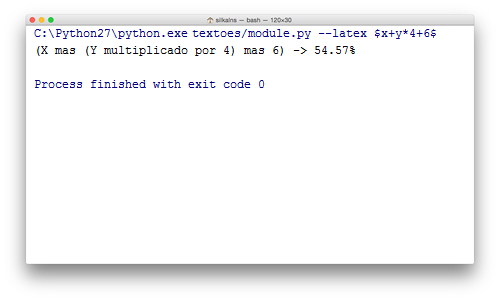
\includegraphics[width=11cm, height=6.62cm]{Figures/demo_1}
  \caption[]{GDC de una transcripción}
\label{fig:demo_1}
\end{figure}

{\Large \textbf{Evaluador semi-automático (human-in-the-loop)}}\\

Este tipo de evaluadores semi-automáticos (HITL o human-in-the-loop\cite{9}) son evaluadores que requieren la interacción del humano para poder proceder.

La idea detrás de este método es ver si los usuarios de TexToES podrían interpretar y reconstruir la fórmula original que ha sido el input de una verbalización; en analogía con la traducción automática, esto correspondería a evaluar TexToES mediante la retrotraducción o traducción inversa; esta evaluación permite medir la adecuación o fidelidad de la traducción. El procedimiento fue el siguiente:

\begin{itemize}
   \item Se han seleccionado 20 fórmulas latex y se ha estimulado TexToES con ellas obteniendo 20 transcripciones.
   \item Se ha construido una encuesta con estas 20 transcripciones y se les ha pedido a voluntarios que escriban la fórmula matemática asociada a esa transcripción.
   \item Por cada respuesta, se ha reconstruido la fórmula latex.
   \item Se compara de igual a igual las fórmulas latex obtenidas con las fórmulas latex empleadas para obtener las transcripciones
\end{itemize}

Los datos empleados (latex y transcripción) en la encuesta pueden ser encontrados en el Apéndice de esta tesis, como así también las respuestas de los voluntarios.

Esta es la parte donde el humano participa en la evaluación, el resto de la evaluación es automática pero necesita de recolectar resultados a través de humanos.

Por lo tanto queremos ver cómo se comporta TexToES informando una transcripción, vamos a definir para este tipo de evaluación la siguiente métrica GDC.

$$GDC = \sum_{i=1}^{N} \frac{1}{N^2}*count(latex_i==resp_i)$$

Dónde N es la cantidad de transcripciones evaluadas, en este caso fueron 13.\\
$latex_i$ es el i-ésimo latex empleado para obtener la transcripción.\\
$resp_i$ es la respuesta i-ésima (que también es un latex) por parte de los voluntarios.

Cabe mencionar que esta métrica de confianza no es una métrica que habla de una transcripción, sino más bien es una métrica que habla de la confianza del sistema de traducción. La métrica intenta capturar la idea de la proporción de un promedio de respuestas correctas.\\

{\Large \textbf{Evaluador humano}}\\

Se han presentados dos evaluadores que buscan definir la calidad de la transcripción pero, sin embargo, la calidad de la traducción es algo subjetivo y de cierta manera el Gold Standard es tener un juicio humano sobre nuestro sistema. Dado que la salida de este sistema es para un ser humano, es correcto pensar que un ser humano lo evalúe. Por otro lado, en la instancia de evaluación humana están presentes factores propias de la comprensión que le permite al juez identificar posibles errores en la traducción.

Pero para ello se necesita de tener un juez humano que entienda tanto del tipo de entrada (\textbf{source}) como el tipo de salida (\textbf{target}) para poder hacer el juicio subjetivo sobre la traducción, esto implica hacer un juicio subjetivo indicando la calidad de una transcripción para una fórmula matemática dada.

La técnica empleada de medición aquí fue presentar una serie de fórmulas matemáticas con sus respectivas transcripciones y se le pide al juez calificar utilizando una escala de múltiples puntos. Estas calificaciones requiere de un juez que entienda ambos lenguajes.

El juicio puesto en juego es de si \textbf{la transcripción es adecuada para la fórmula}.

Se ha utilizado Google Forms para hacer estas preguntas a los voluntarios, presentando las fórmulas con sus verbalizaciones, y una escala tipo Likert\cite{12} para que indiquen su juicio al respecto.

\begin{figure}[H]
\centering
  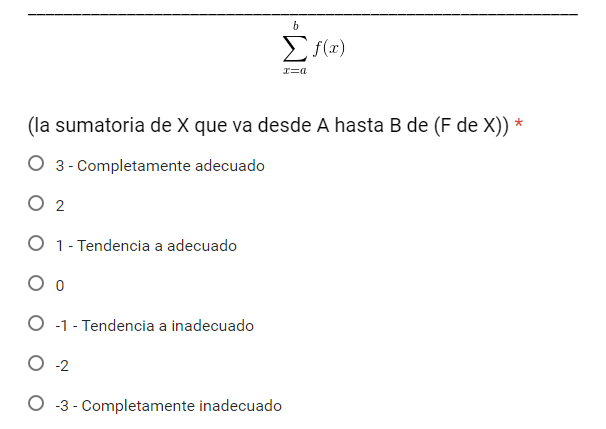
\includegraphics[width=11cm, height=6.62cm]{Figures/evaluadorhumano}
  \caption[]{Evaluador humano}
\label{fig:evaluadorhumano}
\end{figure}

Se han escrito un total de 20 preguntas que muestran las fórmulas matemáticas en imágenes junto a las transcripciones obtenidas con TexToES. Las 20 fórmulas matemáticas intentan contener todo el alcance de TexToES desde sumas, restas hasta sumatorias y aplicación de funciones, y sus combinaciones.

Los resultados obtenidos se muestran en la siguiente sección.


\subsection{Recolección de resultados}

Hemos mostrado varias formas de medir TexToES que buscan estar alineados con el juicio humano, es decir, si un humano dice que la transcripción es buena queremos que nuestros evaluadores digan lo mismo, y así también con los casos en que las transcripciones sean malas. En esta sección se intenta enumerar algunos resultados obtenidos para intentar aplicar correcciones a TexToES para volverlo más natural.

De los tres tipos de métricas que se han elaborado pudimos extraer sugerencias y conocer cómo es que el usuario final suele leer las distintas fórmulas matemáticas.

Para el caso de las encuestas que sirvieron para evaluar las transcripciones automáticamente, aquellas que se le pedía al voluntario cómo leerían un conjunto de fórmulas matemáticas, se han extraído los siguientes patrones.\\

{\Large \textbf{Patrones de traducción}}\\

\begin{itemize}

   \item El 100\% de los encuestados se refiere a la suma entre x e y como \textbf{X más Y}. Por lo tanto la regla de traducción para la etiqueta <plus> debería ser completada con la regla mencionada.
   \item Tanto para el caso de la potencia como para la raíz, el 100\% de los encuestados utilizan \textbf{cuadrado} y \textbf{cubo} para referirse a la aplicación de esas funciones para el 2 y el 3 respectivamente.
   \item Cuando no es la raíz cuadrada ni cúbica, el 100\% de los encuestados utiliza \textbf{raiz X de Y}.
   \item Cuando no es la exponente cuadrada ni cúbica, el 41\% de los encuestados se refiere a \textbf{X a la Y} para mencionar el operador exponencial de X con Y. El 33\% lo menciona como \textbf{X al Y} y el 26\% lo menciona como \textbf{X elevado a Y}
   \item Así como a la suma, para el caso de la resta el 100\% de los encuestados dicen \textbf{X menos Y}.
   \item El 55\% de los encuestados igualan x con y mencionando \textbf{X es igual a Y}, mientras que el resto dicen \textbf{X igual a Y}.
   \item Para el caso de la multiplicación tenemos que el 90\% se refiere a la multiplicación entre x con y como \textbf{X por Y}, mientras que el 10\% restante lo dice como \textbf{X multiplicado por Y}. Es importante notar aquí que TexToES prefiere traducir la multiplicación como\textit{ X multiplicado por Y} haciendo que elija la transcripción menos probable. Una acción a tomar a partir de aquí es cambiar la regla de traducción de TexToES para que elija la más probable.
   \item El 73\% de los encuestados se refieren a la división entre x e y como \textbf{X sobre Y}, mientras que el porcentaje restante elige decir \textbf{X dividido Y}. Cambiar la regla de traducción de TexToES para este caso también hará cambiar las métricas.

\end{itemize}

Estos son algunos datos que podemos extraer de las encuestas realizadas para evaluar a TexToES automáticamente.\\

Algunas sugerencias por partes de los humanos entrevistados para el evaluador semiautomático fueron:
\begin{itemize}
\item Utilizar \textbf{A intersección B}, en lugar de \textbf{A intersectado por el conjunto B} para el caso de la intersección entre dos conjuntos.
\item En la aplicación de la función F en el argumento X, mencionar \textbf{F de X} en lugar de \textbf{F evaluado en X}.
\end{itemize}

Es importante mencionar que estas sugerencias fueron tomadas para modificar la forma de traducir de TexToES, dado que coinciden con la extracción de patrones detalladas en el punto anterior.

Por último, por el lado de la evaluación con juicio humano presentaré aquí algunos resultados.

En total se han recibido una cantidad de \textbf{29 respuestas} para las 20 preguntas que presentaba el Formulario.

Recordemos que cada juez voluntario podía evaluar la transcripción puntuando de la siguiente manera

\begin{itemize}
   \item \textbf{3} \textit{completamente adecuado}
   \item \textbf{2}
   \item \textbf{1} \textit{tendencia a adecuado}
   \item \textbf{0}
   \item \textbf{-1} \textit{tendencia a inadecuado}
   \item \textbf{-2}
   \item \textbf{-3} \textit{completamente inadecuado}
\end{itemize}

Para ayudarnos a interpretar algunos resultados vamos a dividir la tabla de puntos anteriores en tres categorías. La categoría que contiene los puntajes 3, 2 y 1 serán llamados puntajes \textbf{buenos}, para los puntajes marcados como 0 será tratado como puntaje \textbf{neutro} finalmente, para los puntajes de -1, -2 y -3 serán llamados puntajes \textbf{malos}.
Algunos datos interesantes que pueden observarse son:

\begin{itemize}
   \item 9 de 20 transcripciones obtuvieron un puntaje de 3 (completamente adecuado) con más del 70\%
   \item Solo 2 de 20 transcripciones obtuvieron un puntaje entre -3 y -2, y lo obtuvieron como 5\%
   \item 9 de 20 transcripciones obtuvieron solo puntajes buenos
   \item 20 de 20 transcripciones obtuvieron en su mayoría de respuestas puntajes buenos
\end{itemize}

Podemos observar, con la siguiente imagen, que solo una transcripción de las 20 ha obtenido 3 como puntaje en todas sus respuestas asociadas.

\begin{figure}[H]
\centering
  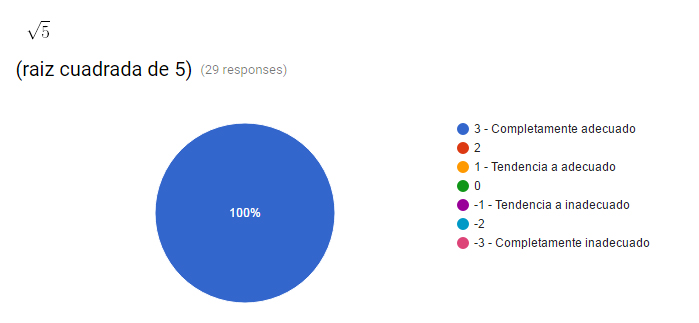
\includegraphics[width=15cm, height=6.93cm]{Figures/captura2}
  \caption[]{Transcripción con 100\% de respuestas en completamente adecuado}
\label{fig:captura2}
\end{figure}

El siguiente es un ejemplo de las 9 transcripciones que ha recibido solo puntaje bueno. Como se puede observar el 100 \% de sus respuestas están en el conjunto de calificaciones buenas (1, 2 o 3)

\begin{figure}[H]
\centering
  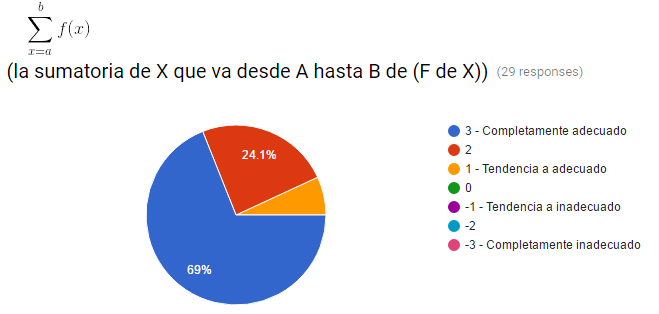
\includegraphics[width=15cm, height=7.15cm]{Figures/captura1}
  \caption[]{Transcripción con solo puntaje bueno}
\label{fig:captura1}
\end{figure}

Y por último, el siguiente es el caso que más respuestas variadas ha tenido y aún así en su mayoría ha obtenido un puntaje bueno. El 69 \% de sus respuestas han incluido 1, 2 y 3 como calificación. Además este también es 1 de las 2 transcripciones que ha obtenido un 3 en el 5\% del total de sus calificaciones.

\begin{figure}[H]
\centering
  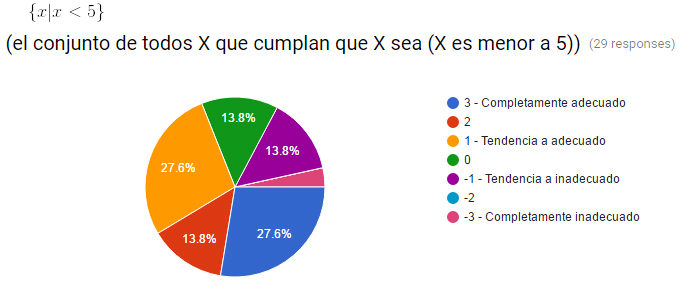
\includegraphics[width=15cm, height=6.39cm]{Figures/captura3}
  \caption[]{Transcripcion con solo puntaje bueno}
\label{fig:captura3}
\end{figure}

Usted puede consultar la lista completa de respuestas en el anexo de este documento.